\documentclass[]{article}
\usepackage{lmodern}
\usepackage{amssymb,amsmath}
\usepackage{ifxetex,ifluatex}
\usepackage{fixltx2e} % provides \textsubscript
\ifnum 0\ifxetex 1\fi\ifluatex 1\fi=0 % if pdftex
  \usepackage[T1]{fontenc}
  \usepackage[utf8]{inputenc}
\else % if luatex or xelatex
  \ifxetex
    \usepackage{mathspec}
  \else
    \usepackage{fontspec}
  \fi
  \defaultfontfeatures{Ligatures=TeX,Scale=MatchLowercase}
\fi
% use upquote if available, for straight quotes in verbatim environments
\IfFileExists{upquote.sty}{\usepackage{upquote}}{}
% use microtype if available
\IfFileExists{microtype.sty}{%
\usepackage{microtype}
\UseMicrotypeSet[protrusion]{basicmath} % disable protrusion for tt fonts
}{}
\usepackage[margin=1in]{geometry}
\usepackage{hyperref}
\hypersetup{unicode=true,
            pdftitle={Filtros de sinais},
            pdfauthor={Amanda Yumi},
            pdfborder={0 0 0},
            breaklinks=true}
\urlstyle{same}  % don't use monospace font for urls
\usepackage{color}
\usepackage{fancyvrb}
\newcommand{\VerbBar}{|}
\newcommand{\VERB}{\Verb[commandchars=\\\{\}]}
\DefineVerbatimEnvironment{Highlighting}{Verbatim}{commandchars=\\\{\}}
% Add ',fontsize=\small' for more characters per line
\usepackage{framed}
\definecolor{shadecolor}{RGB}{248,248,248}
\newenvironment{Shaded}{\begin{snugshade}}{\end{snugshade}}
\newcommand{\KeywordTok}[1]{\textcolor[rgb]{0.13,0.29,0.53}{\textbf{#1}}}
\newcommand{\DataTypeTok}[1]{\textcolor[rgb]{0.13,0.29,0.53}{#1}}
\newcommand{\DecValTok}[1]{\textcolor[rgb]{0.00,0.00,0.81}{#1}}
\newcommand{\BaseNTok}[1]{\textcolor[rgb]{0.00,0.00,0.81}{#1}}
\newcommand{\FloatTok}[1]{\textcolor[rgb]{0.00,0.00,0.81}{#1}}
\newcommand{\ConstantTok}[1]{\textcolor[rgb]{0.00,0.00,0.00}{#1}}
\newcommand{\CharTok}[1]{\textcolor[rgb]{0.31,0.60,0.02}{#1}}
\newcommand{\SpecialCharTok}[1]{\textcolor[rgb]{0.00,0.00,0.00}{#1}}
\newcommand{\StringTok}[1]{\textcolor[rgb]{0.31,0.60,0.02}{#1}}
\newcommand{\VerbatimStringTok}[1]{\textcolor[rgb]{0.31,0.60,0.02}{#1}}
\newcommand{\SpecialStringTok}[1]{\textcolor[rgb]{0.31,0.60,0.02}{#1}}
\newcommand{\ImportTok}[1]{#1}
\newcommand{\CommentTok}[1]{\textcolor[rgb]{0.56,0.35,0.01}{\textit{#1}}}
\newcommand{\DocumentationTok}[1]{\textcolor[rgb]{0.56,0.35,0.01}{\textbf{\textit{#1}}}}
\newcommand{\AnnotationTok}[1]{\textcolor[rgb]{0.56,0.35,0.01}{\textbf{\textit{#1}}}}
\newcommand{\CommentVarTok}[1]{\textcolor[rgb]{0.56,0.35,0.01}{\textbf{\textit{#1}}}}
\newcommand{\OtherTok}[1]{\textcolor[rgb]{0.56,0.35,0.01}{#1}}
\newcommand{\FunctionTok}[1]{\textcolor[rgb]{0.00,0.00,0.00}{#1}}
\newcommand{\VariableTok}[1]{\textcolor[rgb]{0.00,0.00,0.00}{#1}}
\newcommand{\ControlFlowTok}[1]{\textcolor[rgb]{0.13,0.29,0.53}{\textbf{#1}}}
\newcommand{\OperatorTok}[1]{\textcolor[rgb]{0.81,0.36,0.00}{\textbf{#1}}}
\newcommand{\BuiltInTok}[1]{#1}
\newcommand{\ExtensionTok}[1]{#1}
\newcommand{\PreprocessorTok}[1]{\textcolor[rgb]{0.56,0.35,0.01}{\textit{#1}}}
\newcommand{\AttributeTok}[1]{\textcolor[rgb]{0.77,0.63,0.00}{#1}}
\newcommand{\RegionMarkerTok}[1]{#1}
\newcommand{\InformationTok}[1]{\textcolor[rgb]{0.56,0.35,0.01}{\textbf{\textit{#1}}}}
\newcommand{\WarningTok}[1]{\textcolor[rgb]{0.56,0.35,0.01}{\textbf{\textit{#1}}}}
\newcommand{\AlertTok}[1]{\textcolor[rgb]{0.94,0.16,0.16}{#1}}
\newcommand{\ErrorTok}[1]{\textcolor[rgb]{0.64,0.00,0.00}{\textbf{#1}}}
\newcommand{\NormalTok}[1]{#1}
\usepackage{graphicx,grffile}
\makeatletter
\def\maxwidth{\ifdim\Gin@nat@width>\linewidth\linewidth\else\Gin@nat@width\fi}
\def\maxheight{\ifdim\Gin@nat@height>\textheight\textheight\else\Gin@nat@height\fi}
\makeatother
% Scale images if necessary, so that they will not overflow the page
% margins by default, and it is still possible to overwrite the defaults
% using explicit options in \includegraphics[width, height, ...]{}
\setkeys{Gin}{width=\maxwidth,height=\maxheight,keepaspectratio}
\IfFileExists{parskip.sty}{%
\usepackage{parskip}
}{% else
\setlength{\parindent}{0pt}
\setlength{\parskip}{6pt plus 2pt minus 1pt}
}
\setlength{\emergencystretch}{3em}  % prevent overfull lines
\providecommand{\tightlist}{%
  \setlength{\itemsep}{0pt}\setlength{\parskip}{0pt}}
\setcounter{secnumdepth}{0}
% Redefines (sub)paragraphs to behave more like sections
\ifx\paragraph\undefined\else
\let\oldparagraph\paragraph
\renewcommand{\paragraph}[1]{\oldparagraph{#1}\mbox{}}
\fi
\ifx\subparagraph\undefined\else
\let\oldsubparagraph\subparagraph
\renewcommand{\subparagraph}[1]{\oldsubparagraph{#1}\mbox{}}
\fi

%%% Use protect on footnotes to avoid problems with footnotes in titles
\let\rmarkdownfootnote\footnote%
\def\footnote{\protect\rmarkdownfootnote}

%%% Change title format to be more compact
\usepackage{titling}

% Create subtitle command for use in maketitle
\newcommand{\subtitle}[1]{
  \posttitle{
    \begin{center}\large#1\end{center}
    }
}

\setlength{\droptitle}{-2em}

  \title{Filtros de sinais}
    \pretitle{\vspace{\droptitle}\centering\huge}
  \posttitle{\par}
    \author{Amanda Yumi}
    \preauthor{\centering\large\emph}
  \postauthor{\par}
      \predate{\centering\large\emph}
  \postdate{\par}
    \date{29 de setembro de 2018}


\begin{document}
\maketitle

\section{Introdução:}\label{introducao}

O processo de filtragem de sinais permite a caracterização dos sinais a
partir de suas características. Por exemplo, ao aplicar um filtro no
processo de equalização de ondas sonora, podemos verificar que as
frequências mais altas representam os sons mais agudos, enquanto que as
frequências mais baixas representam os sons mais graves.

Outro exemplo é a luz branca, que é a composição de diversas ondas com
diferentes frequências. Assim, ao aplicarmos um filtro podemos separar
as cores individualmente, a partir da aplicação de um filtro de
frequência na cor associada.

Nos casos do sinais de Eletroencefalografia (EEG), temos o ruído da rede
elétrica que no Brasil é 60 Hz. Além desses existem outros artefatos
como ondas de baixas frequências devido ao calor na cabeça do indivíduo.
Deste modo, é extremamente importante aplicação de filtros nestes sinais
para remoção de tais artefatos antes de qualquer outra análise.

Como tirar as baixas e altas frequências pensando em janela de médias?
Podemos definir um filtro passa baixa a partir da subtração do sinal
original pela média aritmética dos pontos ao redor de um ponto. Como
resultado resta no sinal apenas as baixas frequências. Já para um filtro
passa alta, fazemos a subtração do sinal original pelo sinal resultante
do filtro passa baixa. Como resultado resta no sinal apenas os sinais
com alta frequência. Alguns conceitos importantes para a construção dos
filtros:

\begin{itemize}
\tightlist
\item
  \textbf{Frequência de amostragem:} Corresponde ao número de observação
  em um intervalo de tempo. Quando se trabalha com segundo, temos essa
  média em Hz.

  \begin{itemize}
  \tightlist
  \item
    Ex: Na câmera fotográfica temo 30 frames por segundo (fps). Na
    ressonância magnética funcional (fMRI), temos 1 imagem a cada 2
    segundos. Logo, a frequência de amostragem é 1/2 = 0.5Hz
  \item
    Observação: A frequência = 1/período da observação
  \end{itemize}
\item
  \textbf{Frequência de Nyquist:} Corresponde à metade da frequência da
  taxa amostragem.

  \begin{itemize}
  \tightlist
  \item
    Note: A frequência de Nyquist vale para qualquer modalidade de
    técnica de neuroiumagem (fMRI,EEG,fNIRS\ldots{}).
  \end{itemize}
\end{itemize}

O filtro permite a passagem o sinal de parte dos dados e impede a
retirada de outros. São os filtros:

\begin{itemize}
\item
  Passa-alta (\emph{High pass}): Deixa passar as altas frequências
  (maior importância pra alta frequência e baixa importáncia para baixa
  frequência.
\item
  Passa-baixa (\emph{Low pass}): Deixa passar as baixas frequências e dá
  pouca importância às altas frequências.
\item
  Passa-banda (\emph{band pass}): O sinal resultante após o filtro
  possui apenas a banda de frequência utilizada no filtro.
\end{itemize}

\subsection{Implementação de filtros em R e carregando
dados:}\label{implementacao-de-filtros-em-r-e-carregando-dados}

No R faremos primeiro o desenho do filtro: ou seja definir qual o tipo
de frequências vamos passar, para isso usaremos o comando ``butter'' no
pacote signal.

Caso não tenha o pacote, utilize os comandos:

Instalando pacote de sinais no R: * install.packages(``signal'')

e no código chamar a blbioteca

\begin{Shaded}
\begin{Highlighting}[]
\KeywordTok{require}\NormalTok{(signal)}
\end{Highlighting}
\end{Shaded}

O exercício da aula mostra a leitura de um banco de dados de sinais de
EEG.

Para isso, será necessário realizar a leitura dos dados:

\begin{Shaded}
\begin{Highlighting}[]
\NormalTok{sinais=}\KeywordTok{read.table}\NormalTok{(}\StringTok{"oddball250hz.txt"}\NormalTok{,}\DataTypeTok{header=}\OtherTok{FALSE}\NormalTok{)}
\end{Highlighting}
\end{Shaded}

ver também a verificação dos dados:

\begin{Shaded}
\begin{Highlighting}[]
\KeywordTok{dim}\NormalTok{(sinais)}
\end{Highlighting}
\end{Shaded}

\begin{verbatim}
## [1] 45461    33
\end{verbatim}

Olhan do o arquivo, ele é composto por 45461 linhas e 33 colunas (essas
referentes aos 32 canais e uma última coluna de zeros).

Para verificar os dados do arquivo em um plot:

\begin{Shaded}
\begin{Highlighting}[]
\CommentTok{# Plot da série temporal:}
\CommentTok{#gambiarra para o ts.plot funcionar no R Studio:}
\KeywordTok{graphics.off}\NormalTok{()}
\KeywordTok{par}\NormalTok{(}\StringTok{"mar"}\NormalTok{)}
\end{Highlighting}
\end{Shaded}

\begin{verbatim}
## [1] 5.1 4.1 4.1 2.1
\end{verbatim}

\begin{Shaded}
\begin{Highlighting}[]
\KeywordTok{par}\NormalTok{(}\DataTypeTok{mar=}\KeywordTok{c}\NormalTok{(}\DecValTok{1}\NormalTok{,}\DecValTok{1}\NormalTok{,}\DecValTok{1}\NormalTok{,}\DecValTok{1}\NormalTok{))}
\end{Highlighting}
\end{Shaded}

e o plot:

\begin{Shaded}
\begin{Highlighting}[]
\CommentTok{# Plotando gráfico de linha}
\KeywordTok{ts.plot}\NormalTok{(sinais)}
\end{Highlighting}
\end{Shaded}

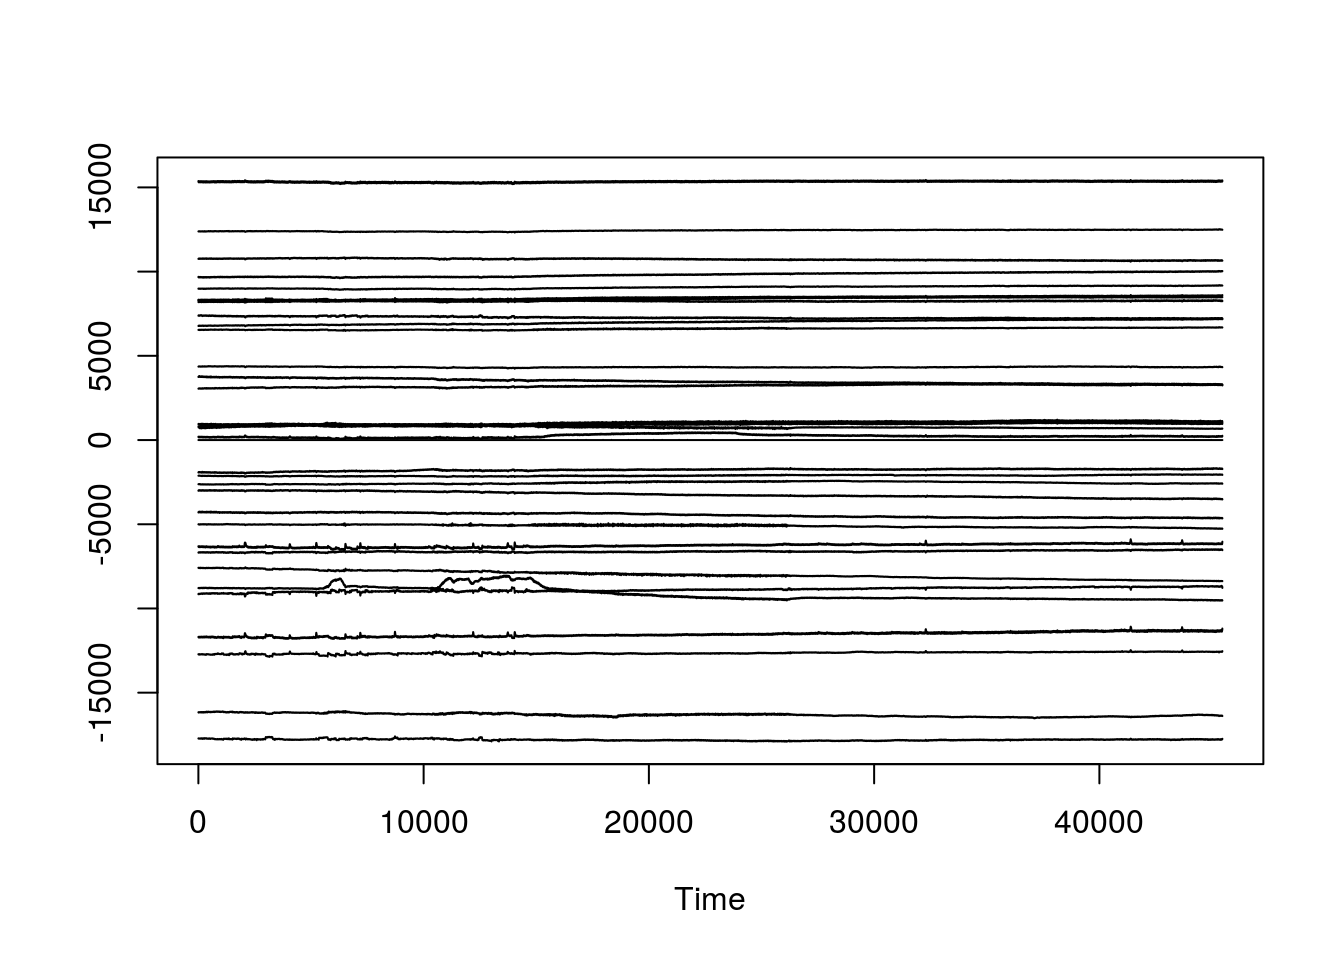
\includegraphics{2_Filtro_Sinais_files/figure-latex/unnamed-chunk-5-1.pdf}

A taxa de amostragem é a frequência em que a leitura ocorre: *
HZ=1/INTERVALO, onde 1hz = 1/s

\begin{Shaded}
\begin{Highlighting}[]
\CommentTok{# Suponha que o sinal foi adquirido sob uma taxa de amostragem de 250Hz: }
\NormalTok{HZ=}\StringTok{ }\DecValTok{250}
\end{Highlighting}
\end{Shaded}

Dessa forma, analisamos o sinal com base nessa amostragem, para todas as
linhas, para o canal 5, com o plot do tipo l (linha):

\begin{Shaded}
\begin{Highlighting}[]
\CommentTok{#Fazer gráfico com frescura:}
\CommentTok{# plot(1:nrow(sinais), sinais[,5],type="l")}
\CommentTok{# mas preciso considerar a frequência convertendo pra segundos:}
\KeywordTok{plot}\NormalTok{((}\DecValTok{1}\OperatorTok{:}\KeywordTok{nrow}\NormalTok{(sinais))}\OperatorTok{/}\NormalTok{HZ, sinais[,}\DecValTok{5}\NormalTok{], }\DataTypeTok{type=}\StringTok{"l"}\NormalTok{, }\DataTypeTok{xlab=}\StringTok{"Tempo(s)"}\NormalTok{, }\DataTypeTok{ylab=} \StringTok{"sinal uV"}\NormalTok{)}
\end{Highlighting}
\end{Shaded}

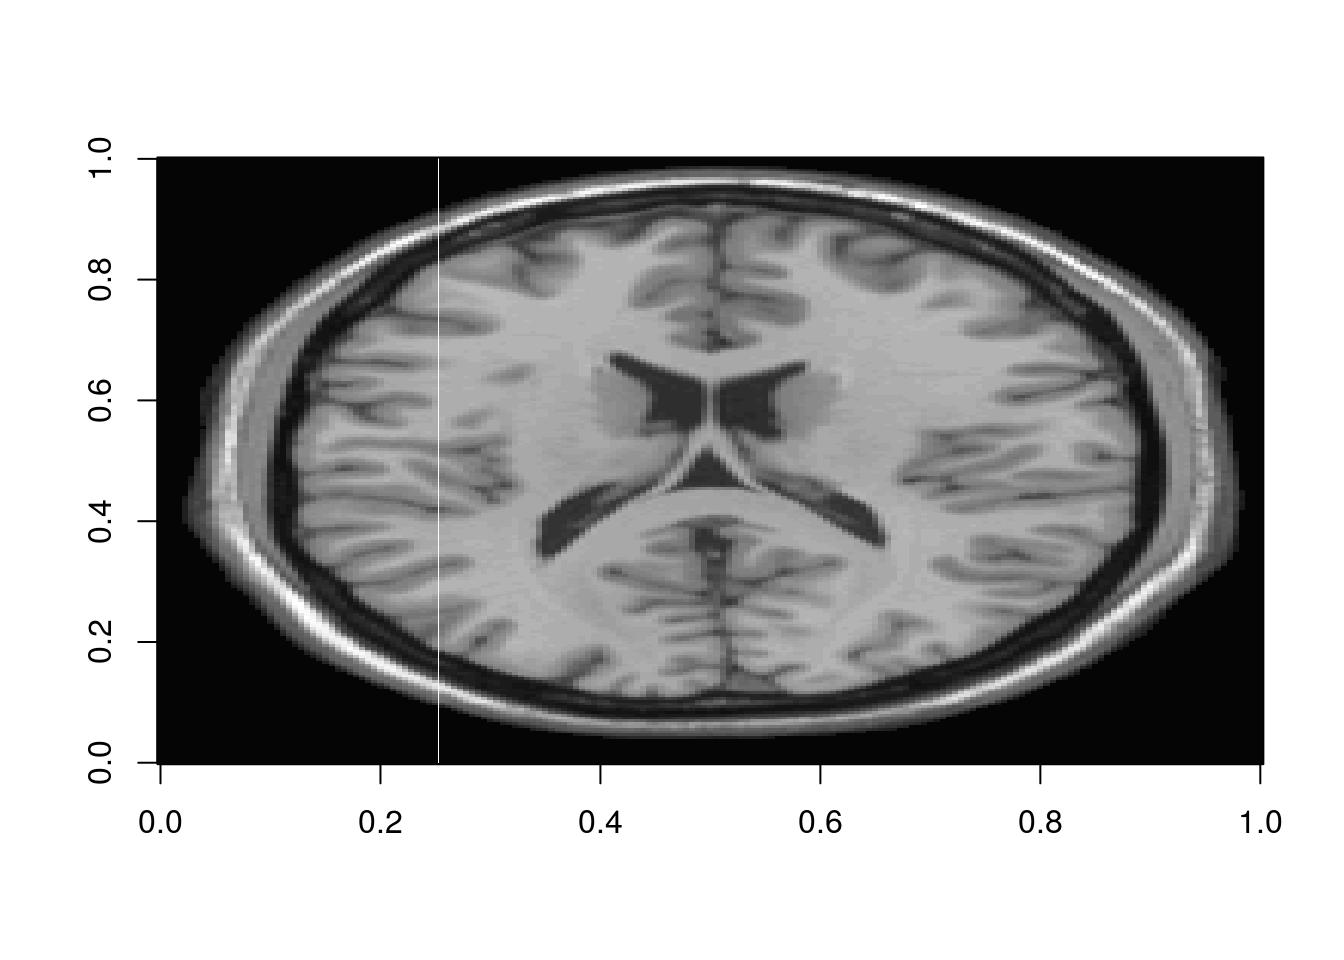
\includegraphics{2_Filtro_Sinais_files/figure-latex/unnamed-chunk-7-1.pdf}

\subsection{\texorpdfstring{Utilizando a função do filtro
(\emph{butter}):}{Utilizando a função do filtro (butter):}}\label{utilizando-a-funcao-do-filtro-butter}

Primeiramente se define qual o tipo de frequências vamos passar, para
isso usaremos o comando ``butter''. A função butter possui a seguinte
síntaxe: * \emph{butter} (n = ordem do filtro, w = cutoff, tipo = tipo
de filtro) onde, + ordem do filtro = controla o decaimento da curva de
ajuste do filtro, geralmente se usa 3 ou 5. + cutoff = frequências que
se queira cortar (é um número de 0 a 1, neste caso é preciso fazer uma
regra de 3; 0 = 1 e 1= frequências de Nyquist) + type = tipo de filtro
(low/passa-baixa, high/passa-alta ou band-pass/passa banda)

Aplicando passa-baixa em 30Hz:

\begin{Shaded}
\begin{Highlighting}[]
\NormalTok{FILTRO =}\StringTok{ }\KeywordTok{butter}\NormalTok{(}\DataTypeTok{n=}\DecValTok{5}\NormalTok{, }\DataTypeTok{W =}\DecValTok{30}\OperatorTok{/}\NormalTok{(HZ}\OperatorTok{/}\DecValTok{2}\NormalTok{), }\DataTypeTok{type =} \StringTok{"low"}\NormalTok{)}

\CommentTok{# Gráfico do desenho do filtro:}
\KeywordTok{freqz}\NormalTok{(FILTRO)}
\end{Highlighting}
\end{Shaded}

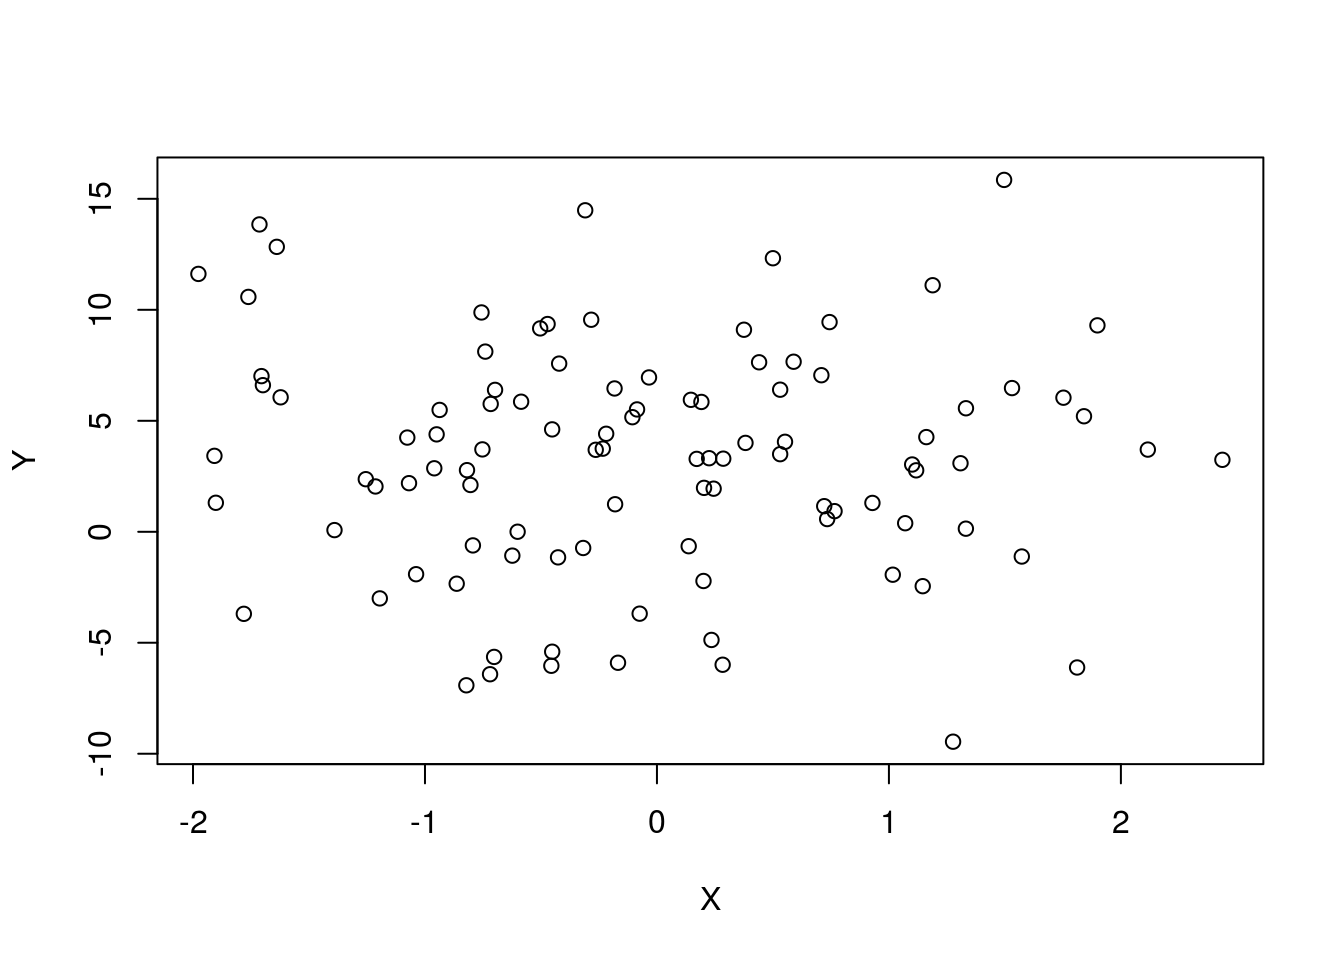
\includegraphics{2_Filtro_Sinais_files/figure-latex/unnamed-chunk-8-1.pdf}

Após ter o filtro desenhado, aplica-lo sobre os dados do canal (neste
caso seria o canal 5, como exemplo, mas poderia ser qlq um). Ao aplicar
o filtro de forma direta teríamos ainda um problema:

\begin{Shaded}
\begin{Highlighting}[]
\NormalTok{filtrado_teste =}\StringTok{ }\KeywordTok{filter}\NormalTok{(FILTRO, sinais[,}\DecValTok{5}\NormalTok{]) }
\CommentTok{# bug de início do sinal, com valor muito alto.}
\end{Highlighting}
\end{Shaded}

Neste caso ``bugado'' teríamos o seguinte retorno:

\begin{Shaded}
\begin{Highlighting}[]
\CommentTok{#Fazer o grafico com os 2 sinais}
\KeywordTok{plot}\NormalTok{((}\DecValTok{1}\OperatorTok{:}\KeywordTok{nrow}\NormalTok{(sinais))}\OperatorTok{/}\NormalTok{HZ, sinais[,}\DecValTok{5}\NormalTok{],}\DataTypeTok{type=}\StringTok{"l"}\NormalTok{,}
     \DataTypeTok{xlab=}\StringTok{"Tempo(s)"}\NormalTok{, }\DataTypeTok{ylab=}\StringTok{"sinal(uV)"}\NormalTok{)}

\CommentTok{#Acrescentar linha com o sinal filtrado}
\KeywordTok{lines}\NormalTok{((}\DecValTok{1}\OperatorTok{:}\KeywordTok{nrow}\NormalTok{(sinais))}\OperatorTok{/}\NormalTok{HZ, filtrado_teste, }\DataTypeTok{col=}\DecValTok{2}\NormalTok{)}
\end{Highlighting}
\end{Shaded}

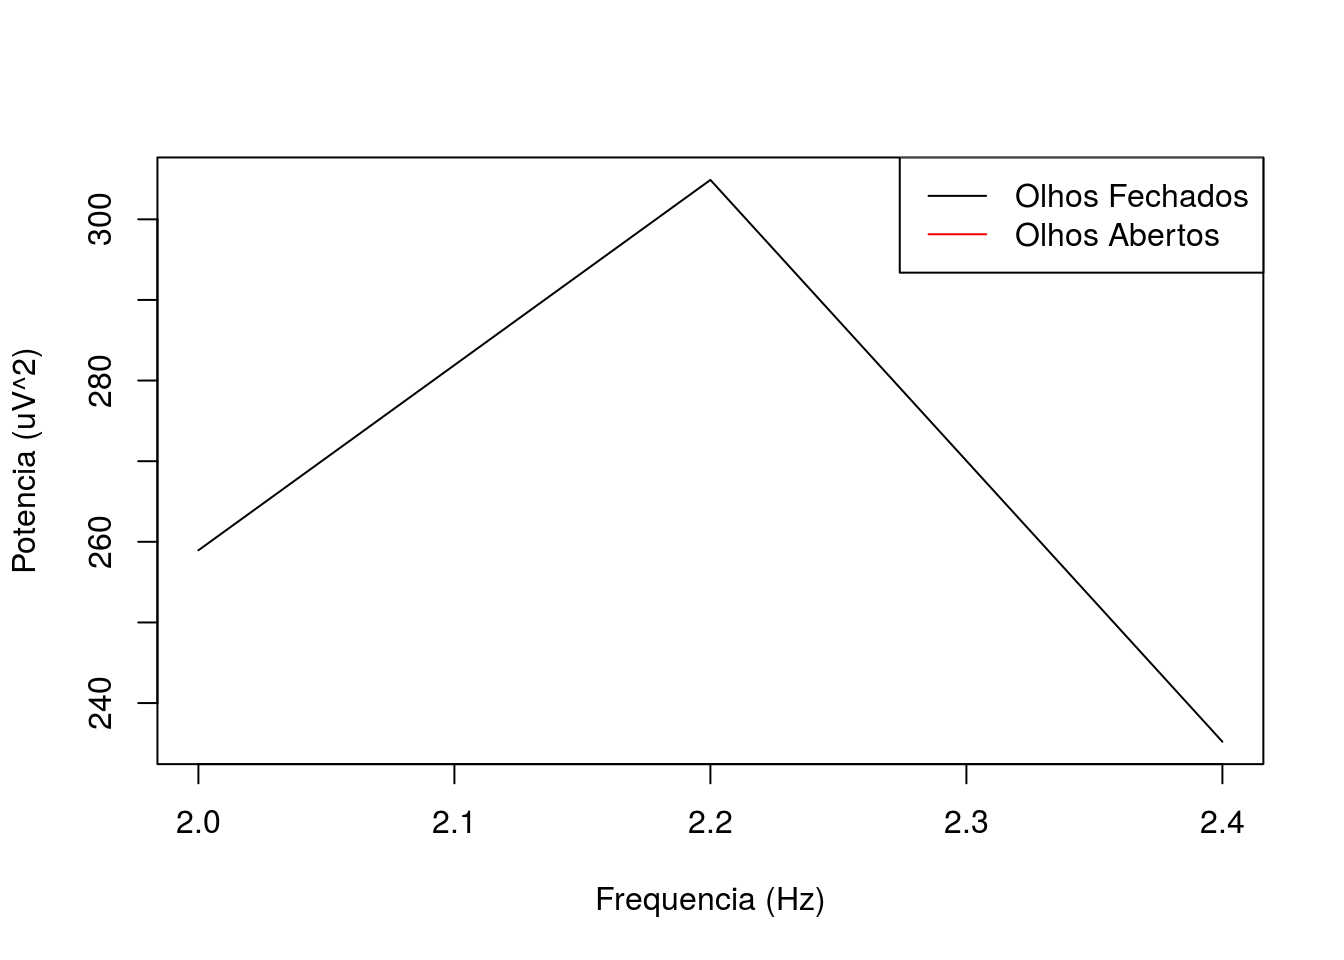
\includegraphics{2_Filtro_Sinais_files/figure-latex/unnamed-chunk-10-1.pdf}

Para isso resolve-se tirando a média do sinal:

\begin{Shaded}
\begin{Highlighting}[]
\NormalTok{y =}\StringTok{ }\NormalTok{sinais[,}\DecValTok{5}\NormalTok{] }\OperatorTok{-}\StringTok{ }\KeywordTok{mean}\NormalTok{(sinais[,}\DecValTok{5}\NormalTok{])}
\CommentTok{# e novamente aplicando o filtro no sinal:}
\NormalTok{filtrado =}\StringTok{ }\KeywordTok{filter}\NormalTok{(FILTRO, y)}
\end{Highlighting}
\end{Shaded}

obtenso então o sinal filtrado:

\begin{Shaded}
\begin{Highlighting}[]
\CommentTok{#Acrescentar linha com o sinal filtrado}
\KeywordTok{plot}\NormalTok{((}\DecValTok{1}\OperatorTok{:}\KeywordTok{nrow}\NormalTok{(sinais))}\OperatorTok{/}\NormalTok{HZ,y,}\DataTypeTok{type=}\StringTok{"l"}\NormalTok{,}
     \DataTypeTok{xlab=}\StringTok{"Tempo(s)"}\NormalTok{, }\DataTypeTok{ylab=}\StringTok{"sinal(uV)"}\NormalTok{)}
\KeywordTok{lines}\NormalTok{((}\DecValTok{1}\OperatorTok{:}\KeywordTok{nrow}\NormalTok{(sinais))}\OperatorTok{/}\NormalTok{HZ, filtrado, }\DataTypeTok{col=}\DecValTok{2}\NormalTok{)}
\end{Highlighting}
\end{Shaded}

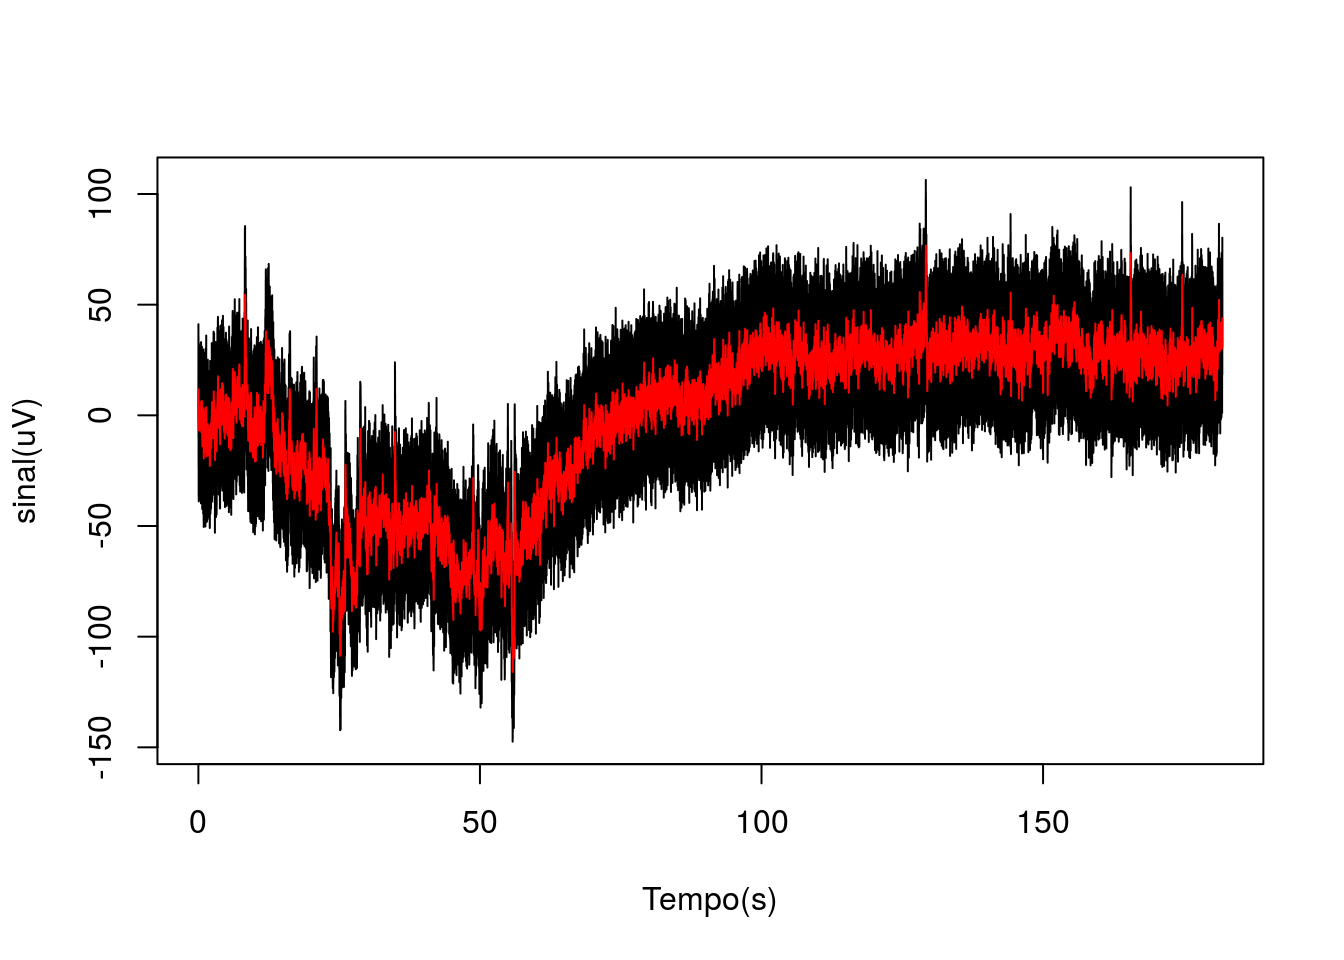
\includegraphics{2_Filtro_Sinais_files/figure-latex/unnamed-chunk-12-1.pdf}

Dessa forma é possível aplicar outros filtros, alterando o tipo na
função \emph{butter} e aplicando aos sinais de todos os canais na função
\emph{filter}. Dica de exercício: Tente executar para outros canais ou
então ajustando o filtro para outras frequências ou determinados
intervalos de frequência.

Um exemplo comum é a aplicação de um filtro que processe dados de um
determinado intervalo (por exemplo, como a rede elétrica é 60hz mas há
oscilações, processa-se sinal entre 59-61hz). Neste caso, queremos um
passa-banda para deixar apenas entre as frequências de 1-40 hz:

\begin{Shaded}
\begin{Highlighting}[]
\CommentTok{# butter (n = ordem do filtro, w = cutoff, tipo = tipo de filtro)}
\CommentTok{#   - n = Ordem do filtro = controla o decaimento da curva de ajuste do filtro, #   geralmente se usa 3 ou 5.}
\CommentTok{#   -type = tipo de filtro (low/passa-baixa, high/passa-alta ou band-pass/passa banda)}

\NormalTok{FILTRO =}\StringTok{ }\KeywordTok{butter}\NormalTok{(}\DataTypeTok{n=}\DecValTok{5}\NormalTok{, }\DataTypeTok{W =}\KeywordTok{c}\NormalTok{(}\DecValTok{1}\NormalTok{,}\DecValTok{40}\NormalTok{)}\OperatorTok{/}\NormalTok{(HZ}\OperatorTok{/}\DecValTok{2}\NormalTok{), }\DataTypeTok{type =} \StringTok{"pass"}\NormalTok{)}
\KeywordTok{freqz}\NormalTok{(FILTRO)}
\end{Highlighting}
\end{Shaded}

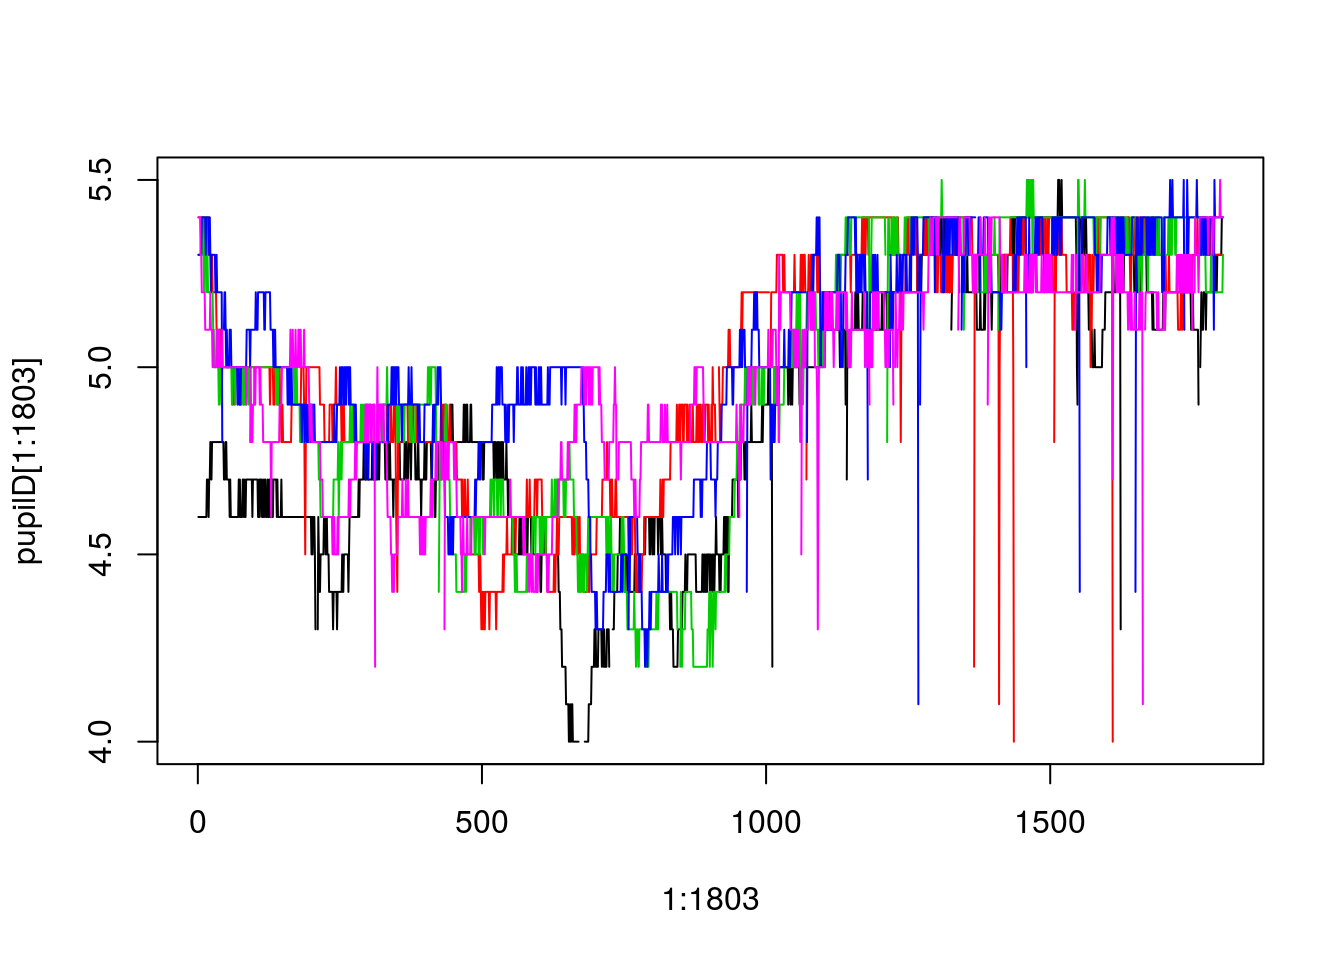
\includegraphics{2_Filtro_Sinais_files/figure-latex/unnamed-chunk-13-1.pdf}

Quero aplicar este filtro em todas as colunas da matriz de sinais,
realizando a retirada da média para tirar os outliers antes do filtro.
Como foi só no y, os sinais brutos continuam com as médias

\begin{Shaded}
\begin{Highlighting}[]
\NormalTok{fsinais =}\StringTok{ }\KeywordTok{matrix}\NormalTok{(}\DecValTok{0}\NormalTok{, }\KeywordTok{nrow}\NormalTok{(sinais), }\KeywordTok{ncol}\NormalTok{(sinais))}

\ControlFlowTok{for}\NormalTok{ (canal }\ControlFlowTok{in} \DecValTok{1}\OperatorTok{:}\DecValTok{32}\NormalTok{) \{}
\NormalTok{  y =}\StringTok{ }\NormalTok{sinais[,canal] }\OperatorTok{-}\StringTok{ }\KeywordTok{mean}\NormalTok{(sinais[,canal])}
\NormalTok{  fsinais[,canal]=}\KeywordTok{filter}\NormalTok{(FILTRO,y)}
\NormalTok{\}}
\end{Highlighting}
\end{Shaded}

Para verificar o sinal bruto e filtrado, tirando a média:

\begin{Shaded}
\begin{Highlighting}[]
\CommentTok{#Checar o sinal bruto e filtrado}
\KeywordTok{plot}\NormalTok{((}\DecValTok{1}\OperatorTok{:}\KeywordTok{nrow}\NormalTok{(sinais))}\OperatorTok{/}\NormalTok{HZ,sinais[,}\DecValTok{1}\NormalTok{]}\OperatorTok{-}\KeywordTok{mean}\NormalTok{(sinais[,}\DecValTok{1}\NormalTok{]),}\DataTypeTok{type=}\StringTok{"l"}\NormalTok{,}\DataTypeTok{xlab=}\StringTok{"Tempo(s)"}\NormalTok{, }\DataTypeTok{ylab=}\StringTok{"sinal(uV)"}\NormalTok{)}
\KeywordTok{lines}\NormalTok{((}\DecValTok{1}\OperatorTok{:}\KeywordTok{nrow}\NormalTok{(sinais))}\OperatorTok{/}\NormalTok{HZ,fsinais[,}\DecValTok{1}\NormalTok{],}\DataTypeTok{col=}\DecValTok{2}\NormalTok{)}
\end{Highlighting}
\end{Shaded}

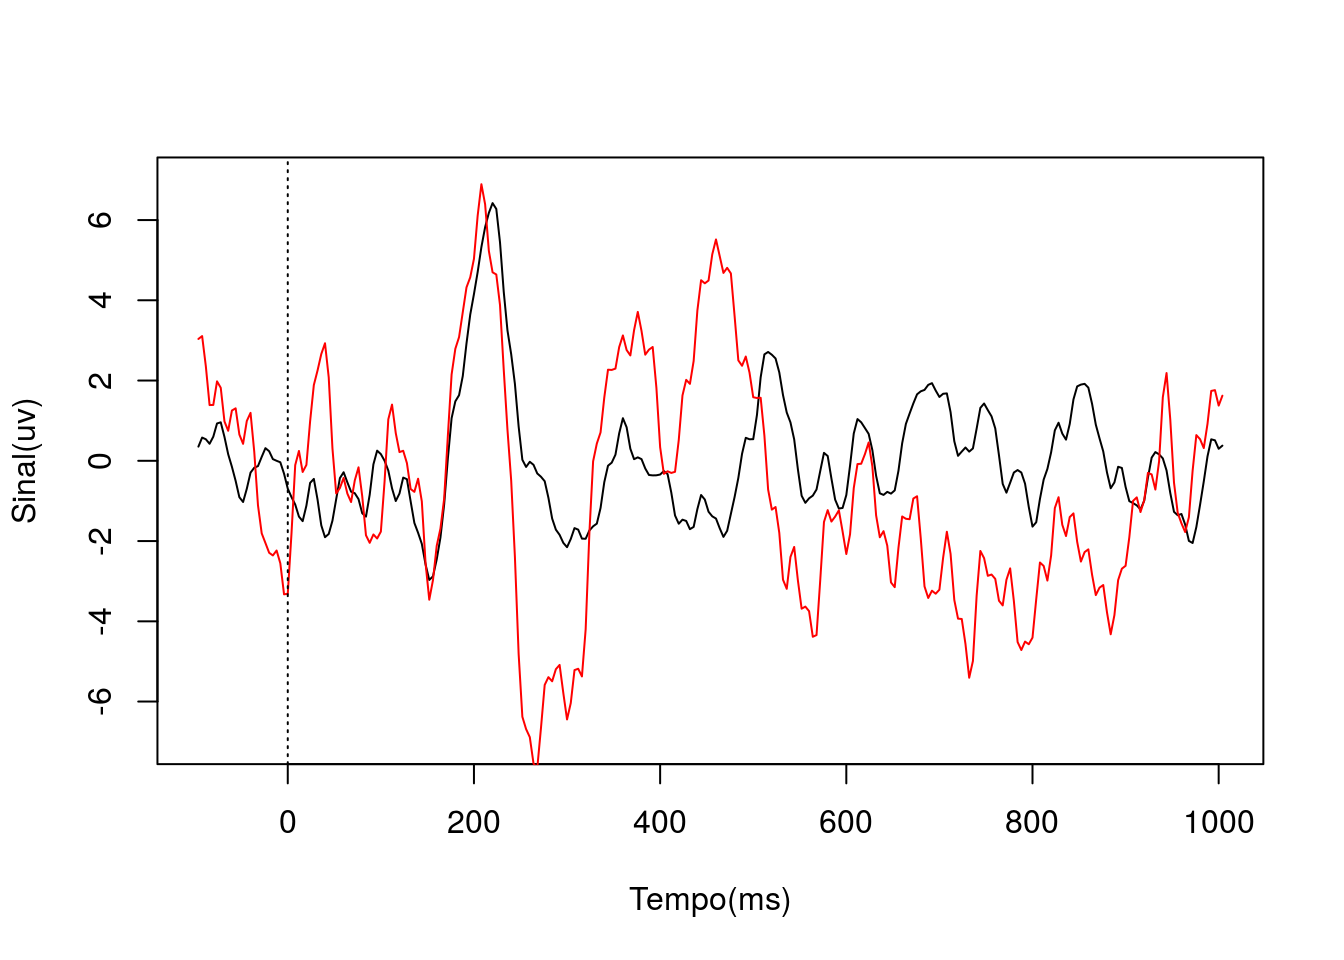
\includegraphics{2_Filtro_Sinais_files/figure-latex/unnamed-chunk-15-1.pdf}


\end{document}
